\documentclass{ctexbeamer}

  \mode<presentation>
  {
    \usetheme{CambridgeUS}      % or try Darmstadt, Madrid, Warsaw, ...
    \usecolortheme{default} % or try albatross, beaver, crane, ...
    \usefonttheme{default}  % or try serif, structurebold, ...
    \setbeamertemplate{navigation symbols}{}
    \setbeamertemplate{caption}[numbered]
  } 
  \usepackage{colortbl}
  \usepackage[english]{babel}
  \usepackage[utf8x]{inputenc}
  
  \title[NIPS2017]{Associative Embedding: End-to-End Learning for Joint Detection and Grouping Alejandro}
  
  \author{Alejandro Newell\\}
  
  \institute{\bf University of Michigan}
  %\textsc {Industrial Training Presentation }
  
  \date{$31^{\text{th}}$ May 2018}
  
  \begin{document}
  
  \begin{frame}
    \titlepage
  \end{frame}

  \begin{frame}
    \frametitle{Abstract}
    We introduce associative embedding, a novel method for supervising convolutional neural networks for the task of detection and grouping. A number ofcomputer vision prob- lems can be framed in this manner including multi-person pose estimation, instance segmentation, and multi-object tracking. Usually the grouping ofdetections is achieved with multi-stage pipelines, instead we propose an approach that teaches a network to simultaneously output detections and group assignments. This technique can be easily integrated into any state-of-the-art network architecture that produces pixel-wise predictions. We show how to apply this method to both multi-person pose estimation and instance segmenta- tion and report state-of-the-art performance for multi-person pose on the MPII and MS-COCO datasets.
  \end{frame}
  
  
  \section{Problem}
  
  \begin{frame}{姿态检测:人体关键点检测}
  
  \begin{itemize}
    \item 给定一张包含人的图片,找出其中人的各个关节(Joint),并为不同人的关键点打上不同的标记(颜色)。
  \end{itemize}
  
  % Commands to include a figure:
  \begin{figure}
  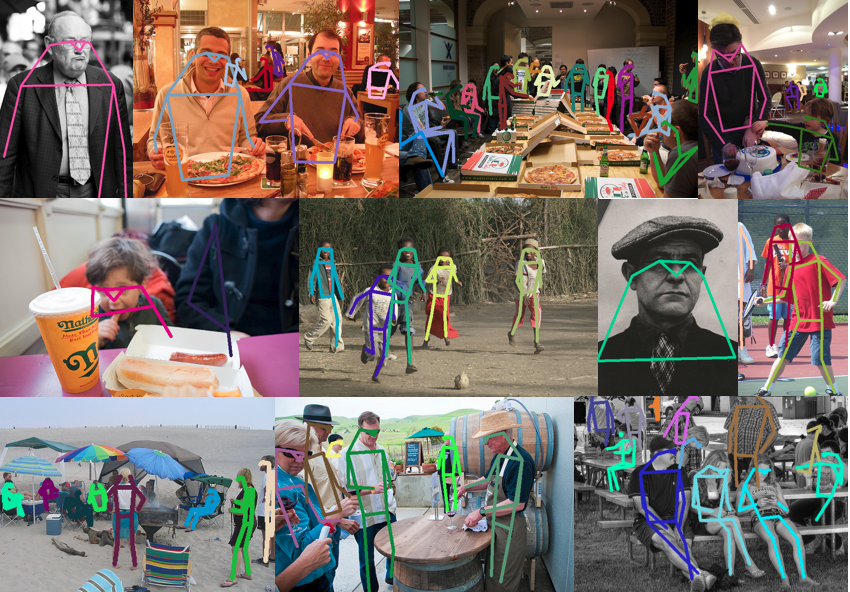
\includegraphics[height= 5cm]{fig/coco-positive.png}
  \caption{\label{fig:pose-detection}Pose-detection}
  \end{figure}
  \vskip 1cm
  
  \end{frame}
  %%%%%%%%%%%%%%%
  
  \section{Related Work}
  
  \begin{frame}{Multiperson Pose Estimation}
  
  \begin{itemize}
    \item Top-down:先检测整个人,然后估计姿态,找出关键点
    \item Bottom-up:先检测独立的关节,然后将关节聚合成一个人
    \item Stacked-Hourglass(单人):Bottom-up与Top-down 结合
    \begin{itemize}
      \item 下采样:多层标准卷积提取关于整图的多组低维特征
      \item 上采样:将多组低维特征组合作为输入,上采样到关键点热力图的尺寸
      \item 重复多层的Hourglass,得到更精确的输出
      \item 回归目标为单个人的关节热力图,每种关节一张图,激活值最高的被选为输出的关键点
    \end{itemize}
  \end{itemize}
  
  % Commands to include a figure:
  \begin{figure}
    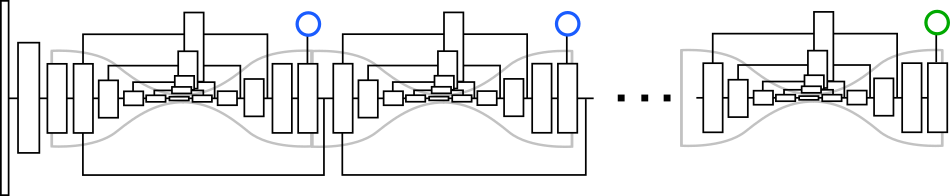
\includegraphics[width=11cm]{fig/stacked-hg-2.png}
    \caption{\label{fig:stack-hourglass}Stacked-Hourglass}
  \end{figure}
  \vskip 1cm
  \end{frame}

  %%%%%%%%%%%%%%%%
  
  \section{Associative embedding}
  
  \begin{frame}{Associative embedding}
  
  \begin{block}{Many computer vision tasks can be viewed as joint detection and grouping}
  \end{block}
  \begin{itemize}
  \item Supervised Regression with Stacked Hourglass Architecture
  \item Detection heatmap:输出每个像素点属于某种joint的概率,每种joint一张heatmap
  \item Associative embedding Tag:输出每种joint的heatmap对应的person tag (论文是每个tag为一个数值,也可以是一个向量)
  \end{itemize}
  
  % Commands to include a figure:
  \begin{figure}
    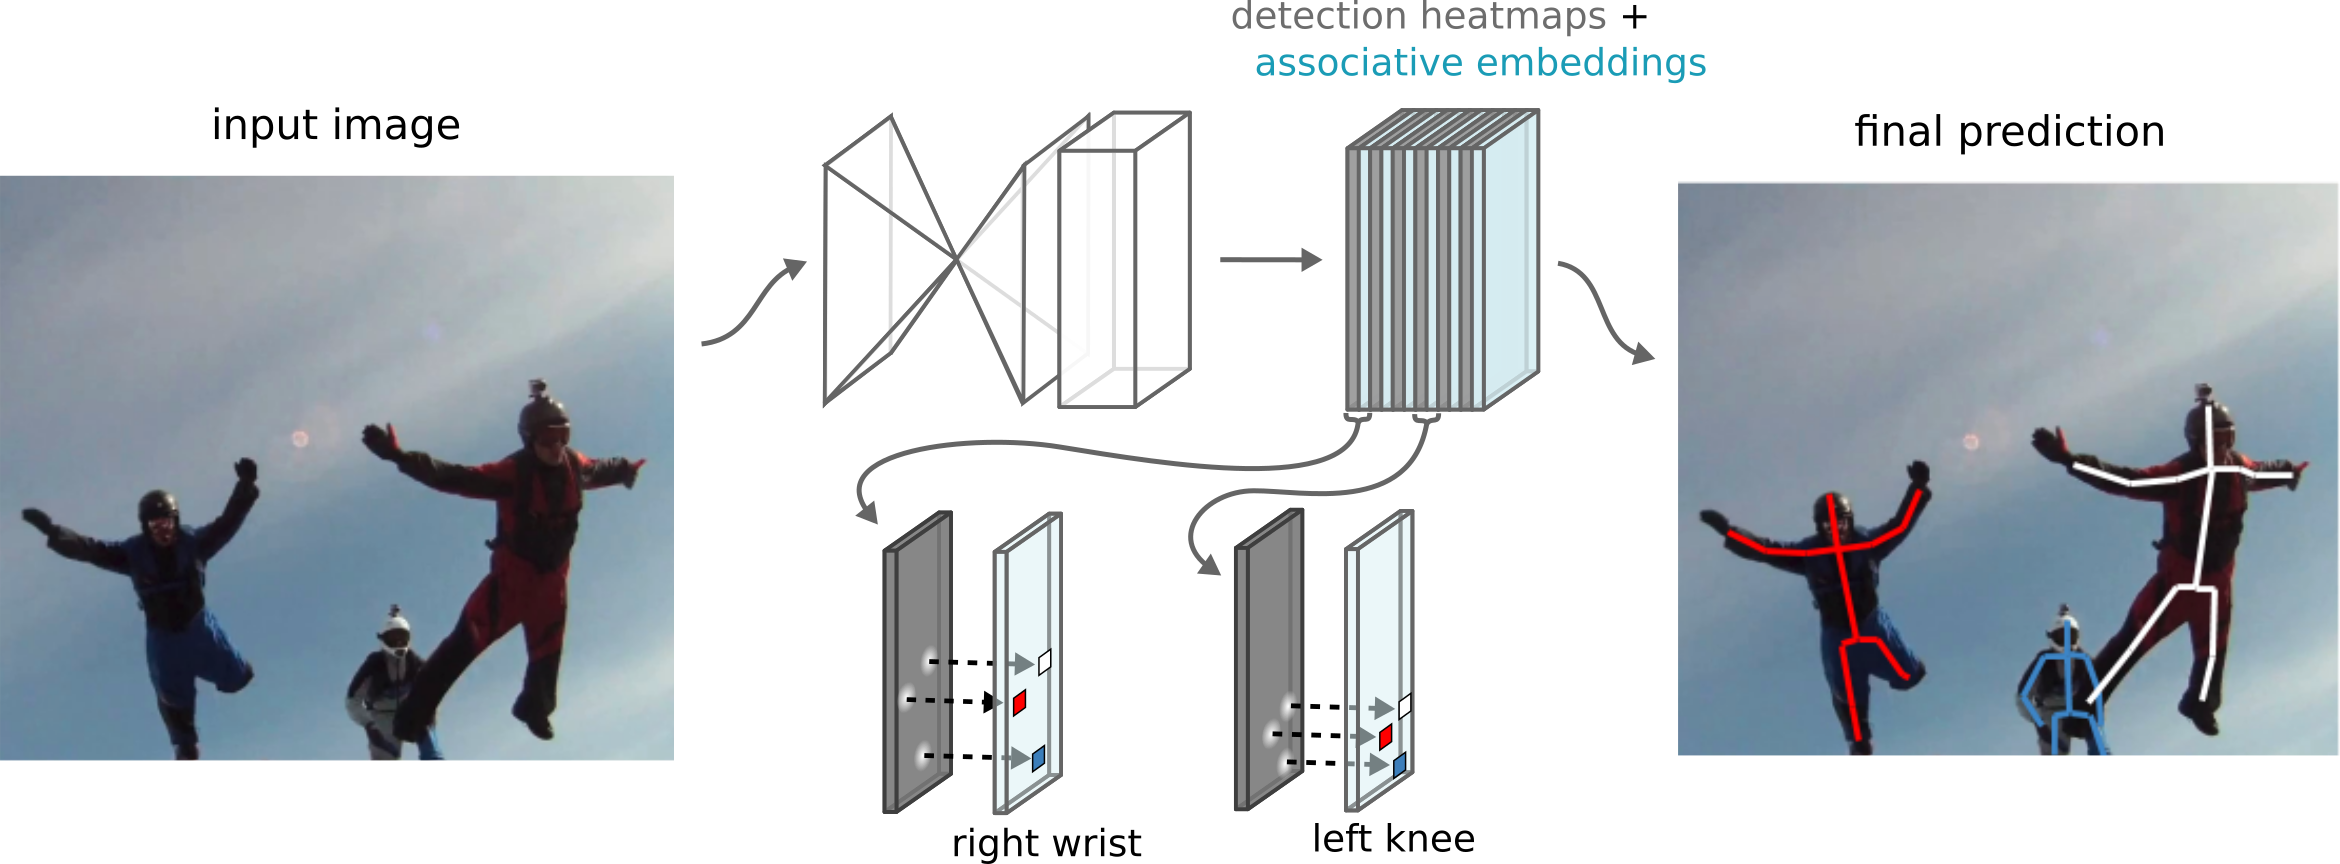
\includegraphics[width=9cm]{fig/ae-overview.png}
    \caption{\label{fig:ae-overview}Associative embedding}
    \end{figure}
  
  \vskip 1cm
  \end{frame}

  \begin{frame}{Modifications on Stacked Hourglass Architecture}
    \begin{itemize}
    \item 增加每个卷积层输出的分辨率(四层分辨率分别为256$\rightarrow$386$\rightarrow$512$\rightarrow$768)
    \item 在Hourglass内部只用3x3卷积,不使用残差模块
    \item 在Hourglass之间保留残差连接,避免深度模型难以训练
    \end{itemize}
    
    % Commands to include a figure:
    \begin{figure}
      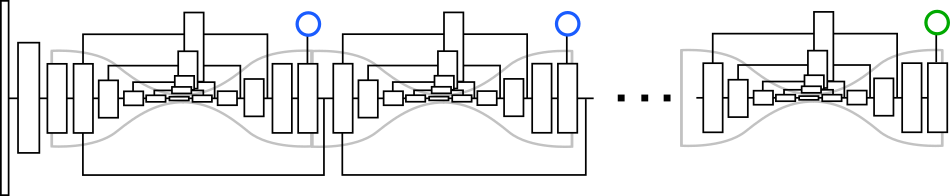
\includegraphics[width=11cm]{fig/stacked-hg-2.png}
    \caption{\label{fig:stack-hourglass-modify}Stacked-Hourglass}
      \end{figure}
    
    \vskip 1cm
    \end{frame}
    \begin{frame}{Training objective}
      \begin{itemize}
      \item 目标:检测出组件,同个人的组件位置和tag要尽量接近,不同人的组件要尽量远离,同时tag尽量不同
      \item Detection loss: $MSE(Heatmap_{pred}, Heatmap_{gt})$
      \begin{itemize}
        \item Groud Truth Heatmap是由关键点图高斯模糊后得到的
        \end{itemize}
      \item Grouping loss: How well the predicted tags agree with the ground truth grouping.
      \end{itemize}
      \vskip 1cm
      \end{frame}

    \begin{frame}{Grouping loss}
      \begin{itemize}
          \item Reference embedding for ith person: $\bar{h}_i=\frac{1}{K}\sum_kh_k(x_{ik})$
          \item $K$是关键点的类别数,$h_k\in R^{W\times H}$是在整张图上预测的tag heatmap, $h(x)$表示在$x$位置的tag value, $x_{ik}$是真实的第i个人第k个关键点的位置. 
          \item 因为两两比较所有关键点的tag太麻烦了,所以先找到关心的位置的tag的均值,作为Reference,让预测值向这个基准靠近
          
      \end{itemize}
      \begin{figure}
        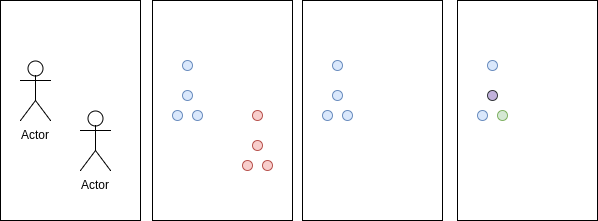
\includegraphics[width=11cm]{fig/hxik.png}
      \caption{\label{fig:hxik} $\bar{h}_i=\frac{1}{K}\sum_kh_k(x_{ik})$}
        \end{figure}
    \vskip 1cm
    \end{frame}
    \begin{frame}{Grouping loss}
      \begin{itemize}
          \item $L_g(h,T)=\frac{1}{N}\sum_i^N\sum_k^K(\bar{h}_i-h_k(x_{ik})^2+\frac{1}{N^2}\sum_i^N\sum_j^{N'}e^{-\frac{1}{2\sigma^2}(\bar{h}_i-\bar{h}_{j})^2}$
          \item $(\bar{h}_i-h_k(x_{ik})^2$将同个人不同关键点的tag向基准拉近
          \item $N'$与当前人不同的人的数量
          \item $e^{-\frac{1}{2\sigma^2}(\bar{h}_i-\bar{h}_{j})^2}$将不同人的tag指数级拉远
      \end{itemize}
      \begin{figure}
        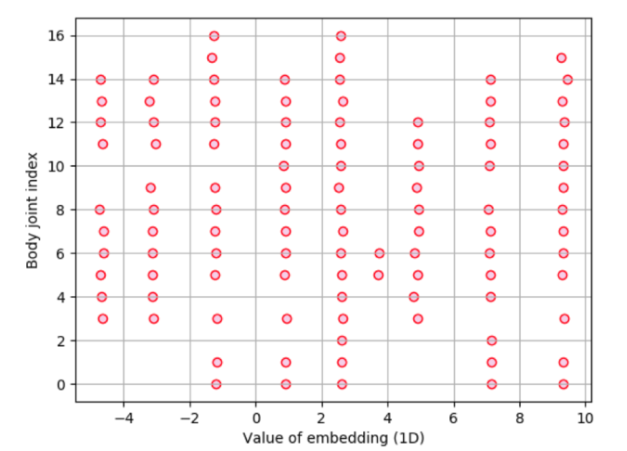
\includegraphics[width=7cm]{fig/value_of_emb.png}
      \caption{\label{fig:value_of_emb} Value of embedding}
        \end{figure}
    \vskip 1cm
    \end{frame}
    \begin{frame}{Testing}
      \begin{itemize}
          
          \item 输出图片的所有关节的heatmap
          \item 对heatmap做非极大抑制,然后保留大于某个阈值的激活点
          \item 输出图片的所有关节heatmap对应的tag heatmap
          \item 从左上到右下遍历不同joint heatmap,将tag差值小于阈值的joint归为同个group
          \item 将输入图片分别拉伸到m个尺度
          \begin{itemize}
            \item 将不同尺度的Detection heatmap求平均
            \item 将不同尺度的tag heatmap做concatenate,每个点得到一个长度为m的tag向量
            \item 计算tag向量之间的相似度来代替单尺度中tag距离判断,其他是一样的
        \end{itemize} 
      \end{itemize}
      \begin{block}{不会像其他pose detection方法那样再去检查修正joint之间的生物空间约束,就已经能达到最好的效果}
      \end{block}
    \vskip 1cm
    \end{frame}    
    
    
  \begin{frame}{Instance Segmentation}
  
    \begin{itemize}
      \item 找到属于不同对象的像素点(像素点级别的分类)
    \end{itemize}
    
    % Commands to include a figure:
    \begin{figure}
      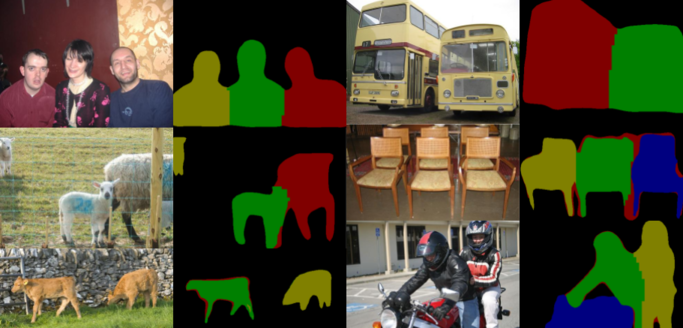
\includegraphics[width=11cm]{fig/inst-exs.png}
      \caption{\label{fig:inst-exs}Instance Segmentation}
      \end{figure}
    \vskip 1cm
    
    \end{frame}
    \begin{frame}{Associative embedding}
  
      \begin{itemize}
        \item Output:
        \begin{itemize}
          \item detection heatmap: 每个元素即每个像素点属于前景的概率,每个类一张heatmap
          \item tag heatmap每个元素即每个像素点所属的具体对象的tag值
        \end{itemize}
        \item Loss
        \begin{itemize}
          \item detection loss: $MSE(Heatmap_{pred}, Heatmap_{mask})$
          \item grouping loss: \\$L_g(h,T) = \sum_i^n\sum_{x\in S_i} \sum_{x'\in S_i} (h(x) - h(x'))^2 + \sum_i^n\sum_i^{n'} \sum_{x\in S_i} \sum_{x'\not\in S_{i}} \exp\{-\frac{1}{2\sigma^2} (h(x) - h(x'))^2\}$
          \item 使得同个instance的关键点线性接近,不同instance的关键点指数拉远
        \end{itemize}
      \end{itemize}
      
      \vskip 1cm
      
      \end{frame}
\section{Experiment}
\begin{frame}
  \frametitle{Datasets}
  \begin{itemize}
  \item MSCOCO2014(现在有2017版了)
  \item MPII(专门做关键点检测的)
 
  \end{itemize}
  \begin{figure}
    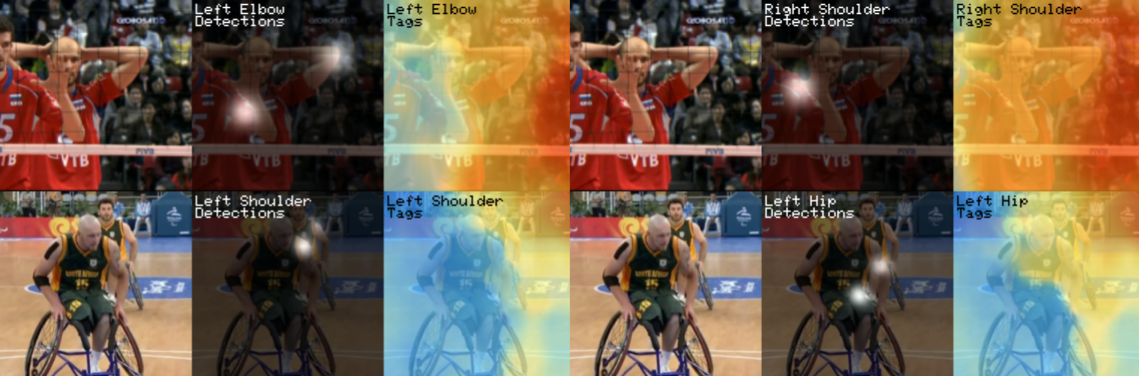
\includegraphics[width=11cm]{fig/hmvis-2.png}
      \caption{\label{fig:hmvis-2}Detection heatmap and Tag heatmap Visualization for different joints}
    \end{figure}

  \vskip 1cm
  \end{frame}
  \begin{frame}
    \frametitle{MAP on key points}
    \begin{figure}
      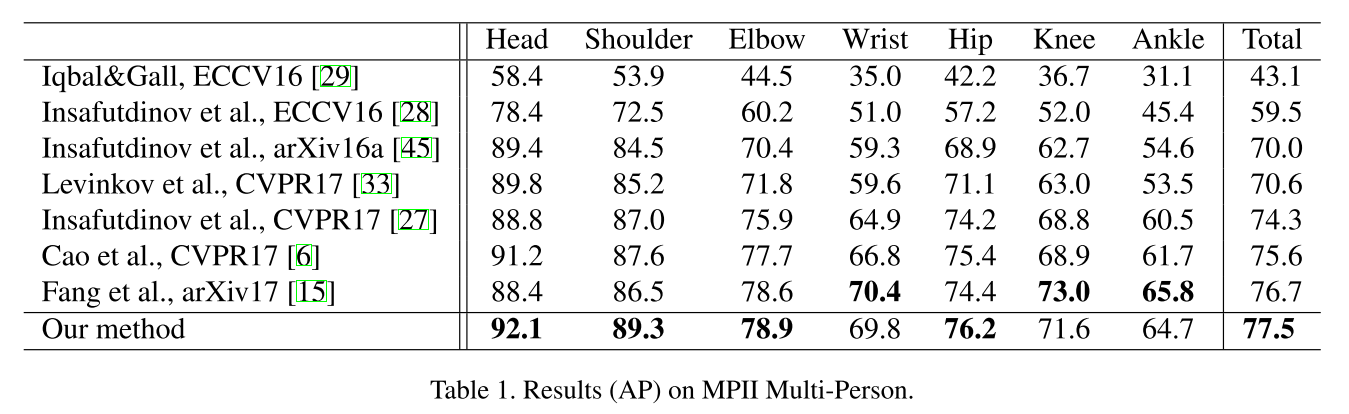
\includegraphics[width=11cm]{fig/table1.png}
        
      \end{figure}
      \begin{figure}
        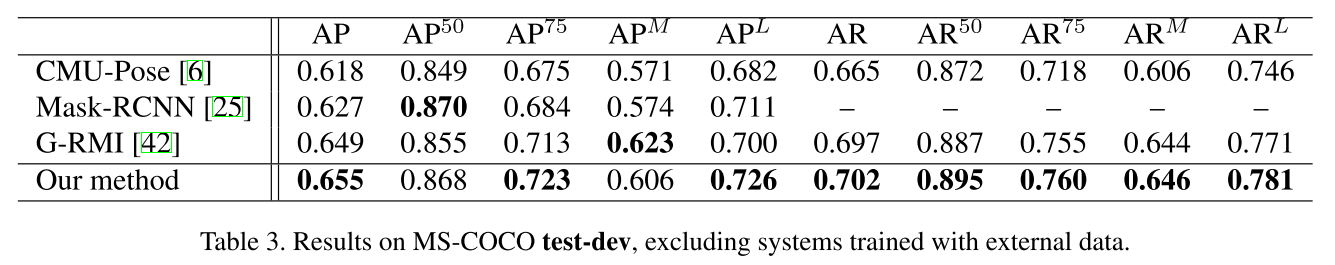
\includegraphics[width=11cm]{fig/table3.png}
          
        \end{figure}
        \vskip 1cm
  \end{frame}
  \begin{frame}
    \frametitle{Evaluation on MSCOO for keypoints}
    \begin{itemize}
      \item  Object keypoint similarity(OKS):$\frac{\sum_i exp(\frac{-d_i^2}{2s^2k_i^2}\delta (v_i>0)}{\sum_i\delta(v_i>0)}$
      \item Average Precision (AP):
      \begin{itemize}
        \item $AP: AP at OKS=.50:.05:.95$ (primary challenge metric) 
        \item $AP^{OKS=.50}$: AP at OKS=.50 (loose metric) 
        \item $AP^{OKS=.75}$ : AP at OKS=.75 (strict metric)
      \end{itemize}
      \item AP Across Scales:
      \begin{itemize}
        \item $AP^{medium}$: AP for medium objects: $32^2 < area < 96^2$
        \item $AP^{large}$: AP for large objects: $area > 96^2$
      \end{itemize}
      
    \end{itemize}
    
  \end{frame}

  \begin{frame}
    \frametitle{Evaluation on MSCOO for keypoints}
    \begin{itemize}
      \item Average Recall (AR):
      \begin{itemize}
        \item $AR: AR at OKS=.50:.05:.95$ (primary challenge metric) 
        \item $AR^{OKS=.50}$: AR at OKS=.50 (loose metric) 
        \item $AR^{OKS=.75}$ : AR at OKS=.75 (strict metric)
      \end{itemize}
      \item AR Across Scales:
      \begin{itemize}
        \item $AR^{medium}$: AR for medium objects: $32^2 < area < 96^2$
        \item $AR^{large}$: AR for large objects: $area > 96^2$
      \end{itemize}
      
    \end{itemize}
    \vskip 1cm
  \end{frame}

  \begin{frame}
    \frametitle{Ablation Study}
    \begin{figure}
      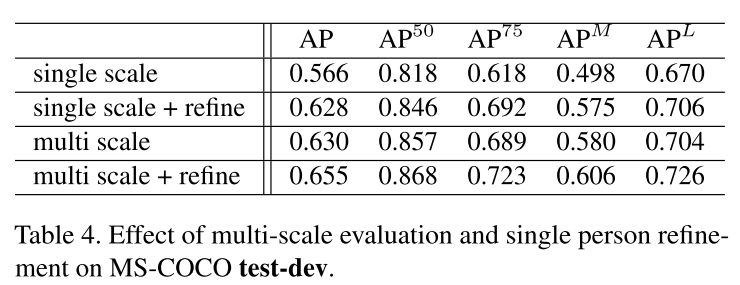
\includegraphics[width=11cm]{fig/table4.png}
      \end{figure}
      \begin{itemize}
        \item Refine: 用一个单人姿态检测器的检测结果修正多人检测结果
        \item 用了多尺度基本就不需要refine了
      \end{itemize}
     \begin{block}{将detection and grouping中的Detection换成ground truth的,用group方法区分keypoints是否属于同个实例,AP $59.2 \rightarrow 94.0$,说明detection是瓶颈}
     \end{block}
    \vskip 1cm
  \end{frame}

  \begin{frame}
    \frametitle{Instance Segmentation Result}
    \begin{figure}
      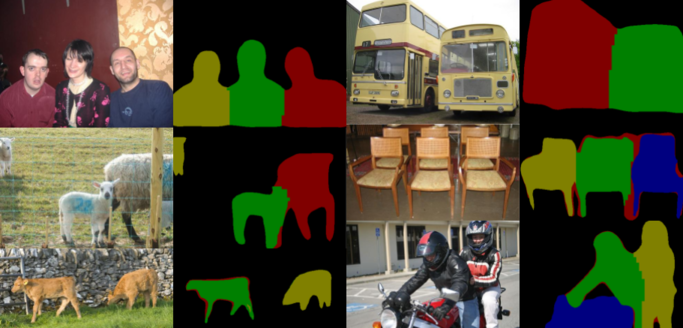
\includegraphics[width=11cm]{fig/inst-exs.png}
      \caption{\label{fig:seg_result}Example instance predictions produced by our system on the PASCAL VOC 2012 validation set.}
      \end{figure}
    \vskip 1cm
  \end{frame}

  \begin{frame}
    \frametitle{Instance Segmentation Result}
    \begin{figure}
      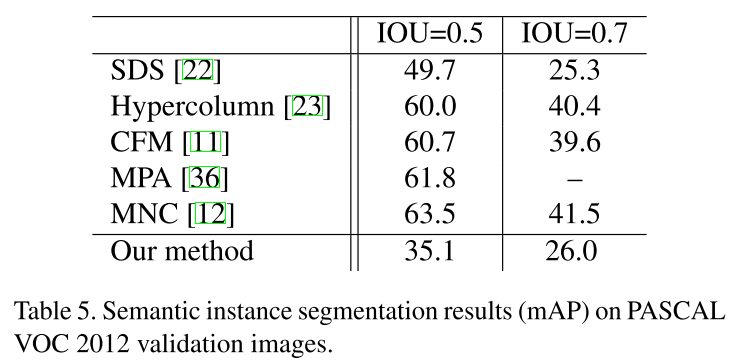
\includegraphics[width=9cm]{fig/table5.png}
      \caption{\label{fig:seg_result}Example instance predictions produced by our system on the PASCAL VOC 2012 validation set.}
      \end{figure}
     \begin{block}{其实效果没有很好,但也是一种可行的方法}
     \end{block}
    \vskip 1cm
  \end{frame}
  %---------------------
  \section{Summary}
  \begin{frame}
  \frametitle{Summary}
  \begin{itemize}
  \item Pose Estimation SOTA
  \item Many computer vision tasks can be viewed as joint detection and grouping
  \end{itemize}
  
  \vskip 1cm
  \end{frame}
  
  \section{References}
  \begin{frame}
  \frametitle{References}
  \begin{itemize}
  \item Associative Embedding: End-to-End Learning for Joint Detection and Grouping. NIPS, 2017.
  \item COCO: Common Objects in Context. \url{http://mscoco. org/home/} \\
  \item Alejandro Newell, Kaiyu Yang, and Jia Deng. Stacked hour- glass networks for human pose estimation. ECCV, 2016. \\
  \end{itemize}
  
  \vskip 1cm
  \end{frame}
  
  \section{End of Presentation}
  \begin{frame}
  \begin{itemize}[<+-| alert@+>]
    % \centering
  \item Thank You.
  \end{itemize}
  \end{frame}
  
  \end{document}
  